%% Template for Master thesis
%% ===========================
%%
%% You need at least KomaScript v3.0.0,
%% e.g. available in Texlive 2009
\documentclass[11pt, a4paper, twoside]{book}
\usepackage[a4paper,left=3cm,right=2cm,top=2.5cm,bottom=2.5cm,bindingoffset=5mm]{geometry}
\usepackage{setspace}

% used pagages
\usepackage[utf8]{inputenc}
\usepackage[T1]{fontenc}
\usepackage[english]{babel}

\usepackage{amsmath}
\usepackage{amssymb}
\usepackage{amsfonts}
\usepackage{slashed}
\usepackage{braket}
\usepackage{mathtools}
\usepackage{bm}

\usepackage{graphicx}
\graphicspath{{./plots/}}
\usepackage{subcaption}

\usepackage{feynmp-auto}

\usepackage{cite}
\bibliographystyle{utphys}
\usepackage{hyperref}

\usepackage{appendix}

% german date setup
\usepackage[ngerman]{datetime}
\newdateformat{myformat}{\THEDAY{ten }\monthnamengerman[\THEMONTH], \THEYEAR}

% colours
\usepackage{color}
\definecolor{darkblue}{rgb}{0.0,0.0,0.4}
\definecolor{darkgreen}{rgb}{0.0,0.4,0.0}

% links
\hypersetup{
    colorlinks,
    linkcolor=black,
    citecolor=darkgreen,
    urlcolor=darkblue
}

\newcommand{\brac}[1] {\!\left(#1\right)}

\begin{document}
\unitlength = 1mm
\pagestyle{empty}


%% this will generate title pages similar to the template provided
%% by the Department of Physics and Astronomy Heidelberg
%%
%% More information:
%% http://www.physik.uni-heidelberg.de/aktuelles/studium/
%% (PDF link: ...studium/download/145/Vorlage_Diplomarbeit_Formular.pdf)

%% Titleintro
\thispagestyle{empty}
\begin{center}
  \renewcommand{\baselinestretch}{2.00}
  \Large\sffamily
  Department of Physics and Astronomy\\
  \large University of Heidelberg
  \par\vfill\normalfont
  Master thesis\\
  in Physics\\
  submitted by\\
  David Conway Lafferty\\
  born in Glasgow\\
  1994
\end{center}
\cleardoublepage

%% Titlepage
\thispagestyle{empty}
\begin{center}
  \renewcommand{\baselinestretch}{2.00}
  \Large\bfseries\sffamily
    (Title)\\
    (of)\\
    (Master thesis)
  \par
  \vfill
  \large\normalfont
  This Master thesis has been carried out by David Conway Lafferty\\
  at the\\
  Institute of Theoretical Physics\\
  under the supervision of\\
  Prof. Dr. Jan M. Pawlowski\\
  \& \\
  Dr. Alexander K. Rothkopf\\
  %% additionally insert second supervisor here if carrying out an
  %% external diploma thesis. Reduce vspace in L. 44 accordingly.
\end{center}\par
\vspace{5\baselineskip}

% reset baselinestretch
\renewcommand{\baselinestretch}{1.00}\normalsize
\cleardoublepage

\cleardoublepage

\pagenumbering{roman}
\pagestyle{plain}

%% Abstract page
%% =============
%%
%% Content of abstract pages has been put into seperate pages to simplify
%% word counting. Use e.g. the unix command
%%   wc abstract-ger.tex
%% or
%%   wc abstract-eng.tex
%% to get the number of words contained in these files.
\thispagestyle{empty}
\begin{center}
  \begin{minipage}[c][0.48\textheight][b]{0.9\textwidth}
    \small
    \textbf{
      (Titel der Masterarbeit - deutsch):
    }\par
    \vspace{\baselineskip}
    %% Latex markup und Zitate funktionieren auch hier
(Abstract in Deutsch, max. 200 Worte. Beispiel: \cite{loremIpsum})

Lorem ipsum dolor sit amet, consectetur adipisici elit, sed eiusmod tempor
incidunt ut labore et dolore magna aliqua. Ut enim ad minim veniam, quis
nostrud exercitation ullamco laboris nisi ut aliquid ex ea commodi consequat.
Quis aute iure reprehenderit in voluptate velit esse cillum dolore eu fugiat
nulla pariatur. Excepteur sint obcaecat cupiditat non proident, sunt in culpa
qui officia deserunt mollit anim id est laborum.

Duis autem vel eum iriure dolor in hendrerit in vulputate velit esse molestie
consequat, vel illum dolore eu feugiat nulla facilisis at vero eros et
accumsan et iusto odio dignissim qui blandit praesent luptatum zzril delenit
augue duis dolore te feugait nulla facilisi. Lorem ipsum dolor sit amet,
consectetuer adipiscing elit, sed diam nonummy nibh euismod tincidunt ut
laoreet dolore magna aliquam erat volutpat.

Ut wisi enim ad minim veniam, quis nostrud exerci tation ullamcorper suscipit
lobortis nisl ut aliquip ex ea commodo consequat. Duis autem vel eum iriure
dolor in hendrerit in vulputate velit esse molestie consequat, vel illum dolore
eu feugiat nulla facilisis at vero eros et accumsan et iusto odio dignissim qui
blandit praesent luptatum zzril delenit augue duis dolore te feugait nulla
facilisi.
  \end{minipage}\par
  \vfill
  \begin{minipage}[c][0.48\textheight][b]{0.9\textwidth}
    \small
    \textbf{
      (Title of Master thesis - english):
    }\par
    \vspace{\baselineskip}
    %% Latex markup and citations may be used here
Lorem ipsum dolor sit amet, consectetur adipisici elit, sed eiusmod tempor
incidunt ut labore et dolore magna aliqua. Ut enim ad minim veniam, quis
nostrud exercitation ullamco laboris nisi ut aliquid ex ea commodi consequat.
Quis aute iure reprehenderit in voluptate velit esse cillum dolore eu fugiat
nulla pariatur. Excepteur sint obcaecat cupiditat non proident, sunt in culpa
qui officia deserunt mollit anim id est laborum.

Duis autem vel eum iriure dolor in hendrerit in vulputate velit esse molestie
consequat, vel illum dolore eu feugiat nulla facilisis at vero eros et
accumsan et iusto odio dignissim qui blandit praesent luptatum zzril delenit
augue duis dolore te feugait nulla facilisi. Lorem ipsum dolor sit amet,
consectetuer adipiscing elit, sed diam nonummy nibh euismod tincidunt ut
laoreet dolore magna aliquam erat volutpat.

Ut wisi enim ad minim veniam, quis nostrud exerci tation ullamcorper suscipit
lobortis nisl ut aliquip ex ea commodo consequat. Duis autem vel eum iriure
dolor in hendrerit in vulputate velit esse molestie consequat, vel illum dolore
eu feugiat nulla facilisis at vero eros et accumsan et iusto odio dignissim qui
blandit praesent luptatum zzril delenit augue duis dolore te feugait nulla
facilisi.
  \end{minipage}
\end{center}


\cleardoublepage

\cleardoublepage

\onehalfspacing 
\tableofcontents

\cleardoublepage

\pagenumbering{arabic}
\chapter{Introduction}
\onehalfspacing 
The strong interaction is the strongest of the four fundamental forces of nature. It is described by quantum chromodynamics (QCD), a quantum field theory exhibiting many peculiar properties. The first, known as asymptotic freedom, is that the underlying interaction strength of QCD decreases as the relevant energy scale increases. Another, which is still not completely understood, is colour confinement -- the phenomenon that the fundamental degrees of freedom of QCD, quarks and gluons, do not exist as isolated objects and instead form bound states known as hadrons. Hadrons make up most of the matter we experience in our everyday lives, and thus colour confinement is observed ubiquitously at the rather mundane energy scales that are naturally present on Earth. However, a more exotic state of matter is theorised to exist at extremely high temperatures or densities -- the Quark Gluon Plasma (QGP). In the QGP, quarks and gluons are considered asymptotically free and no longer confined to within the bounds of a hadron. More generally speaking, the QGP is expected to be one of many regions in the entire phase space of strongly interacting matter, also containing for example the location of neutron stars at high density and low temperature. Indeed, the QGP itself is believed to have existed in the early moments of our universe, and thus understanding its properties will form a crucial part of answering some of the deepest questions of human thought.  

The monumental experimental effort aimed at detecting and quantifying the QGP has culminated today in the relativistic heavy-ion colliders such at those at BNL, CERN, and GSI. The complexity of such experiments has necessitated the development of new techniques both in experiment and theory, in order to firstly map the measured experimental data to QGP properties (a highly non-trivial process) and then to understand how these macroscopic properties emerge from the underlying microscopic theory of QCD. With regards to the former, one refers to various ``probes'' that may indicate the presence of QGP formation. This thesis revolves around one such probe, namely heavy quarkonium.

The bound states of a heavy quark and antiquark of the same flavour are known generically as quarkonia. Since the seminal work of Matsui and Statz \cite{Matsui:1986dk}, the interest in quarkonium as a probe of the QGP has grown into a considerable subfield in the realm of heavy ion collisions. From an experimental perspective, an intricate and not yet fully understood structure has emerged in the production and decay of these mesons throughout the collision process \cite{Aarts:2016hap,Andronic:2015wma}. From the theory side, the development of new effective field theories \cite{Brambilla:2004jw,Brambilla:2000gk,Pineda:2000sz} has allowed quantitative predictions to be made from ever more rigorous formalisms. One such formalism, known as pNRQCD, relies on separating the typical scales present in the system so that the dynamics of the bound state, both in vacuum \cite{Brambilla:2008cx} and at finite temperature \cite{Brambilla:1999xf}, are governed by an effective potential in a non-relativistic Schro{\"o}dinger equation. In this way, the complexities of the full quantum field theory are reduced to a much more tractable quantum mechanical problem.

This thesis presents a new prescription for parametrising the static heavy-quark potential in a background of hot and deconfined charge carriers, such as the QGP. By generalising the Gauss law of classical electromagnetism and combining this with a field-theoretic in-medium permittivity, the resulting in-medium complex potential admits an analytical solution. This can then be used to calculate spectral functions, and give realistic phenomenological predictions. The outline of this thesis is as follows: in Chapter \ref{sec:theory_ov}, we give a short summary of some theoretical aspects of QCD, as well as an introduction into quarkonium phenomenology both in vacuum and in the context of heavy ion collisions. Chapter \ref{sec:med_pot} provides a detailed derivation of the in-medium potential and shows that this parametrisation is able to faithfully reproduce lattice data by utilising only one fitting parameter, the inverse screening length. Chapter \ref{sec:quark_pheno} outlines the procedure with which phenomenologically relevant quantities such as the melting temperatures, decay widths, and electromagnetic decay ratios can be calculated. The main results of this thesis are also given here, and a comparison is made with recent experimental results. A summary and outlook is given in Chapter \ref{sec:conc}. 

%Appendix A contains a short introduction to thermal field theory and in particular the notion of a spectral function. Appendix B gives a more formal derivation of the Debye mass at one-loop order via Euclidean thermal field theory and finally, Appendix C shows how the structure of the in-medium permittivity arises from the Schwinger-Keldysh formalism. 
\chapter{Theory overview}
\label{sec:theory_ov}
\onehalfspacing
In this chapter, we provide the theoretical foundations of various topics that will be important throughout the rest of this thesis. We start with an introduction into quantum chromodynamics, by constructing the Lagrangian and looking at the fundamental interactions. Some more insight will be given on the phenomena of confinement and asymptotic freedom, before a brief discussion of QCD thermodynamics and the phase diagram. We then give an overview of vacuum heavy quarkonium physics by outlining some of the techniques used to discern for example the numerous quantum states in the heavy quark antiquark system. Finally, we introduce some important concepts in heavy ion collisions, with an emphasis on heavy quarkonium phenomenology. 
\section{QCD in vacuum}
In the 1970s, Murray Gell-Mann and George Zweig independently proposed a model to explain the observed spectrum of strongly interacting particles that contained the idea of \emph{quarks} as elementary particles of fractional charge that exist within hadrons. While explaining and predicting the spectrum very well, the quark model contained notable flaws. Namely, the lack of observation of free particles with fractional charge, and the existence of some states apparently in violation of the well-established exclusion principle that quarks, as fermions, must obey. The resolution of the first problem was the introduction of a new, additional quantum number termed \emph{colour}. Each quark would carry one of three possible colour charges -- red, green, or blue, -- the symmetry properties of which mitigated the existence of the problematic states. The second problem was solved by the discovery that non-Abelian gauge theories exhibit asymptotic freedom \cite{Gross:1973id}, which allowed the theory of strong interactions to be brought into its final form. Namely, quantum chromodynamics, a non-Abelian gauge theory with colour symmetry group \(SU\brac{3}\), coupled to quarks acting under the fundamental representation. As is often the case in science, we have had the luxury of summarising decades of previous generations' work in a mere few sentences, glossing over the murky and often enlightening details. For a more detailed historical account of the development of QCD, the reader can consult \cite{Gross:1998jx}.
\subsection{Lagrangian}
\label{sec:QCDLagr}
As a quantum field theory, the fundamental object of QCD is its Lagrangian density (often denoted simply as the Lagrangian), \(\mathcal{L}_{QCD}\), which we now proceed to construct based on the guiding properties outlined in the previous paragraph. The quarks and antiquarks are described respectively by the Dirac spinor fields 
\begin{equation}
\psi_{\alpha,i,f}\brac{x}, \quad\quad \bar{\psi}_{\alpha,i,f}\brac{x},
\end{equation} 
where \(\alpha\) is the spinor index representing the underlying Poincar\'e invariance, \(i=1,2,3\) is the colour index, \(f=1\ldots N_{F}\) labels the flavour quantum number (\(f=\) up, down, strange, charm, bottom, top \(=u,d,s,c,b,t\)), and \(x\) is the position 4-vector. The free quark Lagrangian is then
\begin{equation}
\label{eq:quarklag}
\mathcal{L}_{quark}=\sum_{f}\sum_{i}\bar{\psi}_{\alpha,i,f}\brac{x}\brac{i\brac{\gamma^{\mu}\partial_{\mu}}_{\alpha\beta}-M_{\alpha\beta}}\psi_{\beta,i,f}\brac{x},
\end{equation}
where \(M_{\alpha\beta}=\delta_{\alpha\beta}m_f\) is the quark mass matrix. At this point we impose local gauge invariance as necessitated by the non-Abelian nature of the theory. That is, we require the Lagrangian to remain invariant under the following transformation (neglecting indices):
\begin{equation}
\psi '\brac{x}=U\brac{x}\psi\brac{x},\quad\quad\bar{\psi}'\brac{x}=\bar{\psi}\brac{x}U^\dagger\brac{x},
\end{equation}
where the transformation matrix 
\begin{equation}
U\brac{x}=e^{i\epsilon\left(x\right)}=e^{i\sum\epsilon_a\brac{x} t_a}
\end{equation}
acts on the colour indices. The group parameters are \(\varepsilon_a\brac{x}\) and the group generators, which are the Gell-Mann matrices for \(SU\brac{3}\), are denoted \(t_a\). One can easily verify that the mass term in Eq.~\eqref{eq:quarklag} remains invariant under a gauge transformation, however the spacetime derivative in the kinetic term does not. The resolution is to promote the partial derivative to the covariant derivative 
\begin{equation}
D_\mu=\partial_\mu-igA_\mu
\end{equation}
where the gauge field \(A^\mu\brac{x}=\sum_a A^\mu_a\brac{x}t_a\) is associated to the force-mediating bosons (gluons) and \(g\) is the coupling strength. Local gauge invariance now requires the gluon field to transform as 
\begin{equation}
A_\mu '=UAU^\dagger + \frac{i}{g}U\brac{\partial_\mu U^\dagger}.
\end{equation}
Finally, a kinetic term describing the gluon dynamics is required. The gluon field strength tensor is defined as the commutator of two covariant derivatives:
\begin{equation}
\label{eq:gluonfst}
F_{\mu\nu}\brac{x}=\frac{i}{g}\left[D_\mu,D_\nu \right]=\partial_\mu A\nu - \partial_\nu A_\mu-ig\left[A_\mu,A_\nu\right].
\end{equation}
To see how this structure arises naturally from geometric considerations, the reader can consult \cite{Peskin:1995ev} for an excellent treatment. Eq.~\eqref{eq:gluonfst} transforms as \(F_{\mu\nu}'=UF_{\mu\nu}U^\dagger\), from which we can deduce that a gluon mass term \(\sim m_g A_\mu A^\mu\) would break gauge invariance and hence can not appear in the Lagrangian -- gluons are massless. Contracting two field strength tensors does not lead to a gauge invariant object and one must additionally take the trace in colour space,
\begin{equation}
\mathrm{Tr}\{F'^{\mu\nu}F'_{\mu\nu}\}=\mathrm{Tr}\{F^{\mu\nu}F_{\mu\nu}\}=F^a_{\mu\nu}F_{b}^{\mu\nu}\mathrm{Tr}\{t_at^b\}\sim F^a_{\mu\nu}F_{a}^{\mu\nu}.
\end{equation} 
With this, we are able to write down the QCD Lagrangian in all of its glory. Holding the sum over flavour and colour indices in Eq.~\eqref{eq:quarklag} as implicit, using Feynman slash notation and neglecting the Dirac indices, the Lagrangian takes on the following aesthetically pleasing form:
\begin{equation}
\label{eq:QCD_Lagr}
\mathcal{L}_{QCD}=\bar{\psi}\brac{x}\brac{i\slashed{D}-M}\psi\brac{x}-\frac{1}{4}F^a_{\mu\nu}F_a^{\mu\nu}.
\end{equation}
The above equation is the most fundamental realisation of the strong nuclear force. It is often deemed beautiful that the huge and rich variety of emergent physical phenomena associated with the strong force can be attributed in principle to a single equation. 
\subsection{Running coupling \& asymptotic freedom}
\label{sec:QCD_run_free}
We now proceed to examine the interactions that arise from Eq.~\eqref{eq:QCD_Lagr} at the level of quarks and gluons, and investigate some of their consequences. The first term in Eq.~\eqref{eq:QCD_Lagr} contains a quadratic expression in the fermion field \(\psi\) which describes the propagation of a non-interacting particle. It also couples the fermion field to the gauge field \(A\) through the \(A\) term in the covariant derivative, giving rise to a three-point interaction vertex. Without explicitly expanding the second term, one can easily observe that it will give rise to expressions \(\sim\!A^2, \sim\!A^3\) and \(\sim\!A^4\). The expression quadratic in the gauge fields will eventually describe the propagation of free gluons, although it should be noted here that one must first quantise the theory in a self-consistent way by using the Faddeev-Popov method which is rather non-trivial \cite{Peskin:1995ev}. The expressions \(\sim\!A^3\) and \(\sim\!A^4\) describe gluonic self-interactions. These are unique to QCD as compared to for example the Abelian theory of quantum electrodynamics (QED), and play a vital role in the plethora of highly non-trivial QCD dynamics. The diagrammatic representations of each expression above is given in Fig.~\ref{fig:QCD_tree}. 
\begin{figure}[t]
    \centering
    \begin{subfigure}[b]{0.3\textwidth}
    	\begin{fmffile}{QCDfermion}
    		\begin{fmfgraph}(40,25)
    		\fmfleft{i1}
    		\fmfright{o1}
    		\fmf{vanilla}{i1,o1}
    		\end{fmfgraph}
    	\end{fmffile}
        \caption{Free quark propagator}
    \end{subfigure}
    \begin{subfigure}[b]{0.3\textwidth}
    	\begin{fmffile}{QCDgluon}
    		\begin{fmfgraph}(40,25)
    		\fmfleft{i1}
    		\fmfright{o1}
    		\fmf{gluon}{i1,o1}
    		\end{fmfgraph}
    	\end{fmffile}
        \caption{Free gluon propagator}
    \end{subfigure}
    \vspace*{10mm}

    \begin{subfigure}[b]{0.3\textwidth}
    	\begin{fmffile}{QCDfermglu}
    		\begin{fmfgraph}(40,25)
    		\fmfleft{i1,i2}
    		\fmfright{o1}
    		\fmf{vanilla}{i1,v1}
    		\fmf{vanilla}{i2,v1}
    		\fmf{gluon}{o1,v1}
    		\fmfdot{v1}
    		\end{fmfgraph}
    	\end{fmffile}
        \caption{Quark-gluon vertex}
    \end{subfigure}
    \begin{subfigure}[b]{0.3\textwidth}
    	\begin{fmffile}{QCDglu3}
    		\begin{fmfgraph}(40,25)
    		\fmfleft{i1,i2}
    		\fmfright{o1}
    		\fmf{gluon}{i1,v1}
    		\fmf{gluon}{i2,v1}
    		\fmf{gluon}{o1,v1}
    		\fmfdot{v1}
    		\end{fmfgraph}
    	\end{fmffile}
    	\vspace*{5mm}
        \caption{Cubic gluon vertex}
    \end{subfigure}    
    \begin{subfigure}[b]{0.3\textwidth}
    	\begin{fmffile}{QCDglu4}
    	\begin{fmfgraph}(40,25)
    		\fmfleft{i1,i2}
    		\fmfright{o1,o2}
    		\fmf{gluon}{i1,v1}
    		\fmf{gluon}{i2,v1}
    		\fmf{gluon}{o1,v1}
    		\fmf{gluon}{o2,v1} 	
    		\fmfdot{v1}
    		\end{fmfgraph}
    	\end{fmffile}
    \vspace*{5mm}
    \caption{Quartic gluon vertex}
    \end{subfigure}
    \vspace*{4mm}
    \caption{Tree-level QCD diagrams.}
   	\label{fig:QCD_tree}
\end{figure}

Before being able to quantitatively understand asymptotic freedom, we must first introduce \emph{renormalisation} and the concept of a running coupling. Although it is recognised today that quantum field theory (QFT) is the only consistent framework that can emerge from the union of quantum mechanics and special relativity \cite{weinberg_1996}, this was by no means obvious in its historical development. In the early days, quantum field theoretic tools could be used to describe some physical processes with good accuracy, however its usefulness was certainly not ubiquitous. The theory also exhibited some worrying features -- most notably, the emergence of unphysical infinities when calculating scattering amplitudes beyond leading order. QFT was considered so sick that even its most ardent practitioners acknowledged the need for something of an overhaul, with many physicists advocating employing somewhat different formalisms to describe the most fundamental interactions \cite{Gross:1998jx}.

The remedy eventually came by way of renormalisation. The modern picture is as follows: the expressions describing fundamental processes often contain divergent integral expressions, which are nonetheless able to be quantified and isolated by the process of \emph{regularisation}. Then, the free parameters such as the masses and coupling constant in a Lagrangian like Eq.~\eqref{eq:QCD_Lagr} are interpreted as `bare' and unphysical. They must be split into a physical part and a corresponding unphysical `counter-term' that will cancel the infinities present in the theory. In this way, the divergences are swept under the proverbial rug, leaving the physical parameters that must be measured in experiment. This was seen by some as a cheap trick when first introduced, however with the advent of Kenneth Wilson's renormalisation group originating from statistical physics, it is today valued as an indispensable tool in describing the physical world. In the Wilsonian viewpoint the subtraction of infinity can be seen as an admission of our ignorance, in the sense that we introduce a cut-off scale at large momenta or small distances, beyond which the theory is not expected to hold. The renormalisation group is a fascinating tool that permeates many areas of theoretical physics today, with powerful accompanying ideas and extensions such as universality; the interested reader can refer to \cite{Kopietz:2010zz,Cardy:1996xt}.

One consequence of renormalisation is that the physical parameters inherit a scale dependence. Much like the way in which the spring constant in Newton's second law depends on the make-up of the spring and can only be measured in mechanical experiments, the physical masses and coupling constants of a renormalised quantum field theory will depend on the momentum (or equivalently, distance) scale probed by a particular collider experiment. In the case of a given coupling constant, this phenomenon is known generically as the running of the coupling. One can calculate (via the renormalisation procedure outlined above) to a given order how the coupling constant will change as the momentum scale is changed. This is usually expressed via the beta function
\begin{equation}
\label{eq:betafunc}
\beta\brac{g\brac{Q^2}}=Q^2\frac{\partial g\brac{Q^2}}{\partial Q^2},
\end{equation}
where \(g\) is the physical coupling constant evaluated at momentum scale \(Q^2\) (one should distinguish explicitly between the bare and physical parameters; for the remainder of this thesis we refer to only the physical parameters and in an abuse of notation use the same symbols as in Sec.~\ref{sec:QCDLagr}). For QCD the relevant diagrams at one-loop order are shown in Fig.~\ref{fig:QCDbeta_oneloop} and the result is
\begin{align}
\label{eq:betaQCD_oneloop}
\beta_{QCD}\brac{g}\lvert_{\mathrm{1-loop}}&=-\beta_0\frac{g^3}{16\pi^2}+\mathcal{O}\brac{g^5} \\[1.5ex]
&= -\beta_0\frac{\alpha_S}{2\pi}+\mathcal{O}\brac{\alpha_S^2} \label{eq:betaQCD_oneloop_alpha}
\end{align}
where we have introduced the more commonly used \(\alpha_s=g^2/4\pi\) and
\begin{equation}
\beta_0=\frac{33-2 N_F}{12\pi}
\end{equation}
with \(N_F\) equal to the number of light fermion flavours. The minus sign in Eq.~\eqref{eq:betaQCD_oneloop} is of tremendous importance. It implies that for \(N_F\leq 16\) the physical QCD coupling constant approaches zero as the energy or momentum scale tends to infinity. This phenomenon is known as asymptotic freedom.
\begin{figure}[t]
    \centering
    \begin{subfigure}[b]{0.3\textwidth}
    	\begin{fmffile}{fermionself}
    		\begin{fmfgraph}(40,25)
    		\fmfleft{i1}
    		\fmfright{o1}
    		\fmf{vanilla,tension=3}{i1,v1}
    		\fmf{vanilla,tension=3}{o1,v2}
    		\fmf{vanilla}{v2,v1}
    		\fmf{gluon,left=1}{v1,v2}
    		\fmfdot{v1,v2}
    		\end{fmfgraph}
    	\end{fmffile}
    \end{subfigure}
    \begin{subfigure}[b]{0.3\textwidth}
    	\begin{fmffile}{gluonself4}
    	\begin{fmfgraph}(40,25)
    		\fmfleft{i1}
    		\fmfright{o1}
    		\fmf{gluon}{i1,v1}
    		\fmf{gluon}{v1,v1}
    		\fmf{gluon}{v1,o1}
    		\fmfdot{v1}
    		\end{fmfgraph}
    	\end{fmffile}
    \end{subfigure}
    
    \begin{subfigure}[b]{0.3\textwidth}
    	\begin{fmffile}{gluonself1}
    		\begin{fmfgraph}(40,25)
    		\fmfleft{i}
    		\fmfright{o}
    		\fmf{gluon,tension=3}{i,v1}
    		\fmf{vanilla,left=1}{v1,v2,v1}
    		\fmf{gluon,tension=3}{v2,o}
    		\fmfdot{v1,v2}
    		\end{fmfgraph}
    	\end{fmffile}
    \end{subfigure}
    \begin{subfigure}[b]{0.3\textwidth}
    	\begin{fmffile}{gluonself2}
    		\begin{fmfgraph}(40,25)
    		\fmfleft{i}
    		\fmfright{o}
    		\fmf{gluon,tension=3}{i,v1}
    		\fmf{dashes,left=1}{v1,v2,v1}
    		\fmf{gluon,tension=3}{v2,o}
    		\fmfdot{v1,v2}
    		\end{fmfgraph}
    	\end{fmffile}
    \end{subfigure}
    \begin{subfigure}[b]{0.3\textwidth}
    	\begin{fmffile}{gluonself3}
    		\begin{fmfgraph}(40,25)
    		\fmfleft{i}
    		\fmfright{o}
    		\fmf{gluon,tension=3}{i,v1}
    		\fmf{gluon,left=1}{v1,v2,v1}
    		\fmf{gluon,tension=3}{v2,o}
    		\fmfdot{v1,v2}
    		\end{fmfgraph}
    	\end{fmffile}
    \end{subfigure}   
    \vspace*{10mm}
    
     
    \begin{subfigure}[b]{0.3\textwidth}
    	\begin{fmffile}{vertex1}
    		\begin{fmfgraph}(40,25)
    		\fmfleft{i1,i2}
		    \fmfright{o1}
   			\fmf{plain,tension=1/3}{i1,v2,v1}
   			\fmf{plain,tension=1/3}{i2,v3,v1}
   			\fmf{gluon,tension=0}{v2,v3}
   			\fmf{gluon}{v1,o1}
   			\fmfdot{v1,v2,v3}
    		\end{fmfgraph}
    	\end{fmffile}
    \end{subfigure}
        \begin{subfigure}[b]{0.3\textwidth}
    	\begin{fmffile}{vertex2}
    		\begin{fmfgraph}(40,25)
    		\fmfleft{i1,i2}
		    \fmfright{o1}
   			\fmf{plain,tension=1/3}{i1,v2}
   			\fmf{plain,tension=1/3}{i2,v3}
   			\fmf{gluon,tension=0}{v3,v2}
   			\fmf{gluon,tension=1/3}{v2,v1}
   			\fmf{gluon,tension=1/3}{v1,v3}
   			\fmf{gluon}{v1,o1}
   			\fmfdot{v1,v3,v2}
    		\end{fmfgraph}
    	\end{fmffile}
    \end{subfigure}
    \vspace*{4mm}
    \caption{One-loop running.}
   	\label{fig:QCDbeta_oneloop}
\end{figure}

By integrating Eq.~\eqref{eq:betaQCD_oneloop_alpha}, one can extrapolate the value of the experimentally measured coupling at momentum transfer \(\mu\) to an arbitrary momentum scale \(Q\):
\begin{equation}
\label{eq:gQCD_oneloop}
\alpha_S\brac{Q^2}=\frac{\alpha_S\brac{\mu^2}}{1+\alpha_S\brac{\mu^2}\beta_0\log\frac{Q^2}{\mu^2}}.
\end{equation}
The above equation encompasses the running of the coupling. Note that this expression is only to one-loop order and more accurate calculations would include additional terms in Eq.~\eqref{eq:betaQCD_oneloop_alpha}, however beyond second order the result becomes dependent on the renormalisation scheme employed. Fig.~\ref{fig:RunningCoupling} shows numerical results for the 4-loop calculation. At larger momenta the smallness of the effective coupling permits the use of perturbation theory, which has been incredibly successful in describing high energy scattering processes \cite{Bethke:2006ac}. Conversely, as the low-momenta infrared regime is approached, perturbative methods break down and one must employ other techniques such as lattice gauge theory (see Sec.~\ref{sec:latticeQCD}). One can make this quantitative by defining 
\begin{equation}
\label{eq:|ambdaQCD}
\Lambda_{QCD}^2=\frac{\mu^2}{e^{1/\brac{\beta_0\alpha_s\brac{\mu^2}}}},
\end{equation}
such that Eq.~\ref{eq:gQCD_oneloop} becomes
\begin{equation}
\label{eq:gQCD_oneloop_new}
\alpha_S\brac{Q^2}=\frac{1}{\beta_0\log\frac{Q^2}{\Lambda_{QCD}^2}}.
\end{equation}
In doing so, a dimensionful parameter \(\Lambda_{QCD}\) is introduced such that \(\alpha_S\brac{Q^2}\to\infty\) as \(Q^2\to\Lambda_{QCD}^2\). Thus \(\Lambda_{QCD}\) is an estimate for the momentum scale where non-perturbative dynamics become important. Recent results give \(\Lambda_{QCD}\sim 200\mathrm{MeV}\) \cite{Bethke:2009jm}. It should be stressed here that this picture is purely perturbative -- one should take this calculation to give a clear sign that non-perturbative methods are required, and not a proof that the coupling actually becomes infinite at this scale.
\begin{figure}[t]
	\centering
	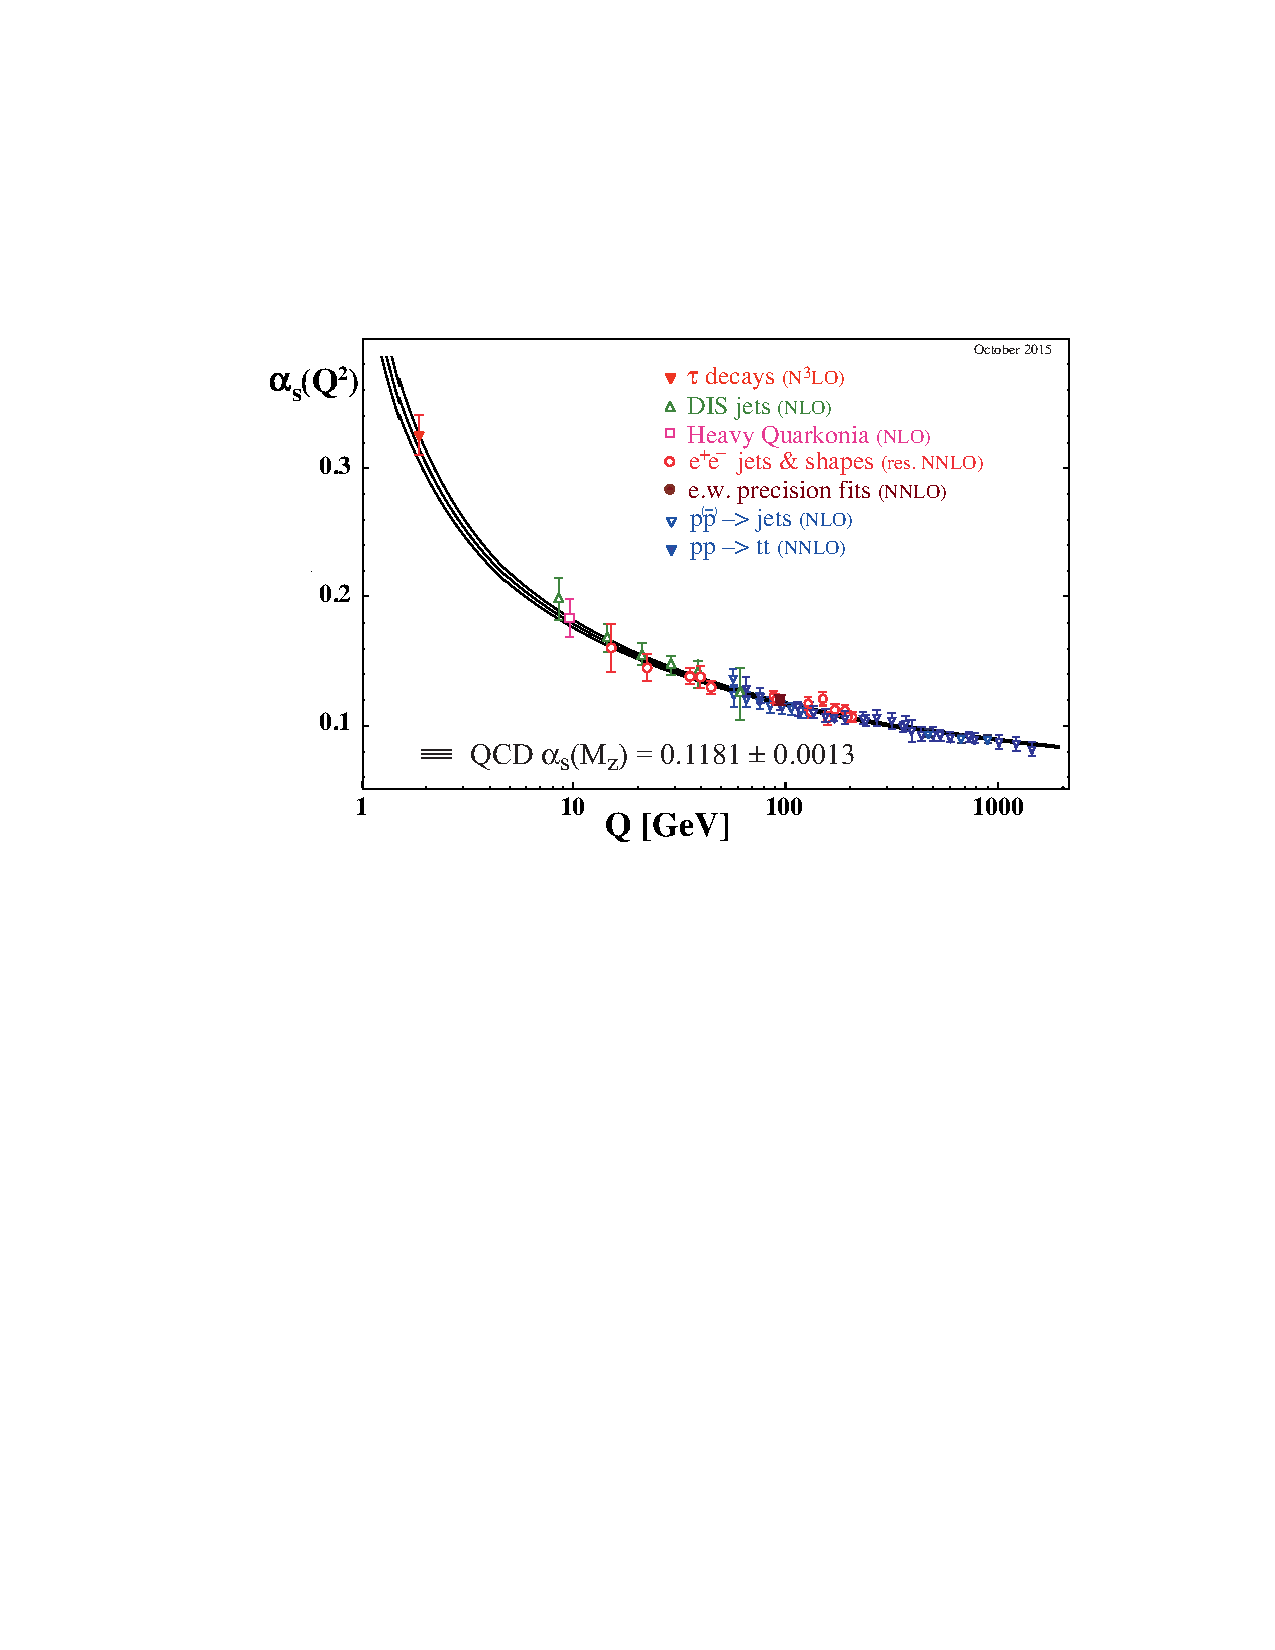
\includegraphics[width=\textwidth]{QCDRunningCoupling}
	\caption{Running coupling \cite{PhysRevD.98.030001}.}\label{fig:RunningCoupling}
\end{figure}
\subsection{Vacuum polarisation}
\label{sec:VacPol}
We now provide a physical picture for the running coupling in terms of vacuum polarisation and (anti-)screening; these ideas will be central throughout the rest of this thesis. The quantum mechanical vacuum is far from an empty place, with virtual particle-antiparticle pairs continually being created and destroyed. In this way, the vacuum behaves as a dynamical medium and exhibits effects such as diamagnetic and paramagnetic behaviour. Inserting a test charge into the medium, the field produced will be modified by this vacuum polarisation so that the experimentally measured charge depends on the distance from which it is measured.
\begin{figure}[t]
	\centering
	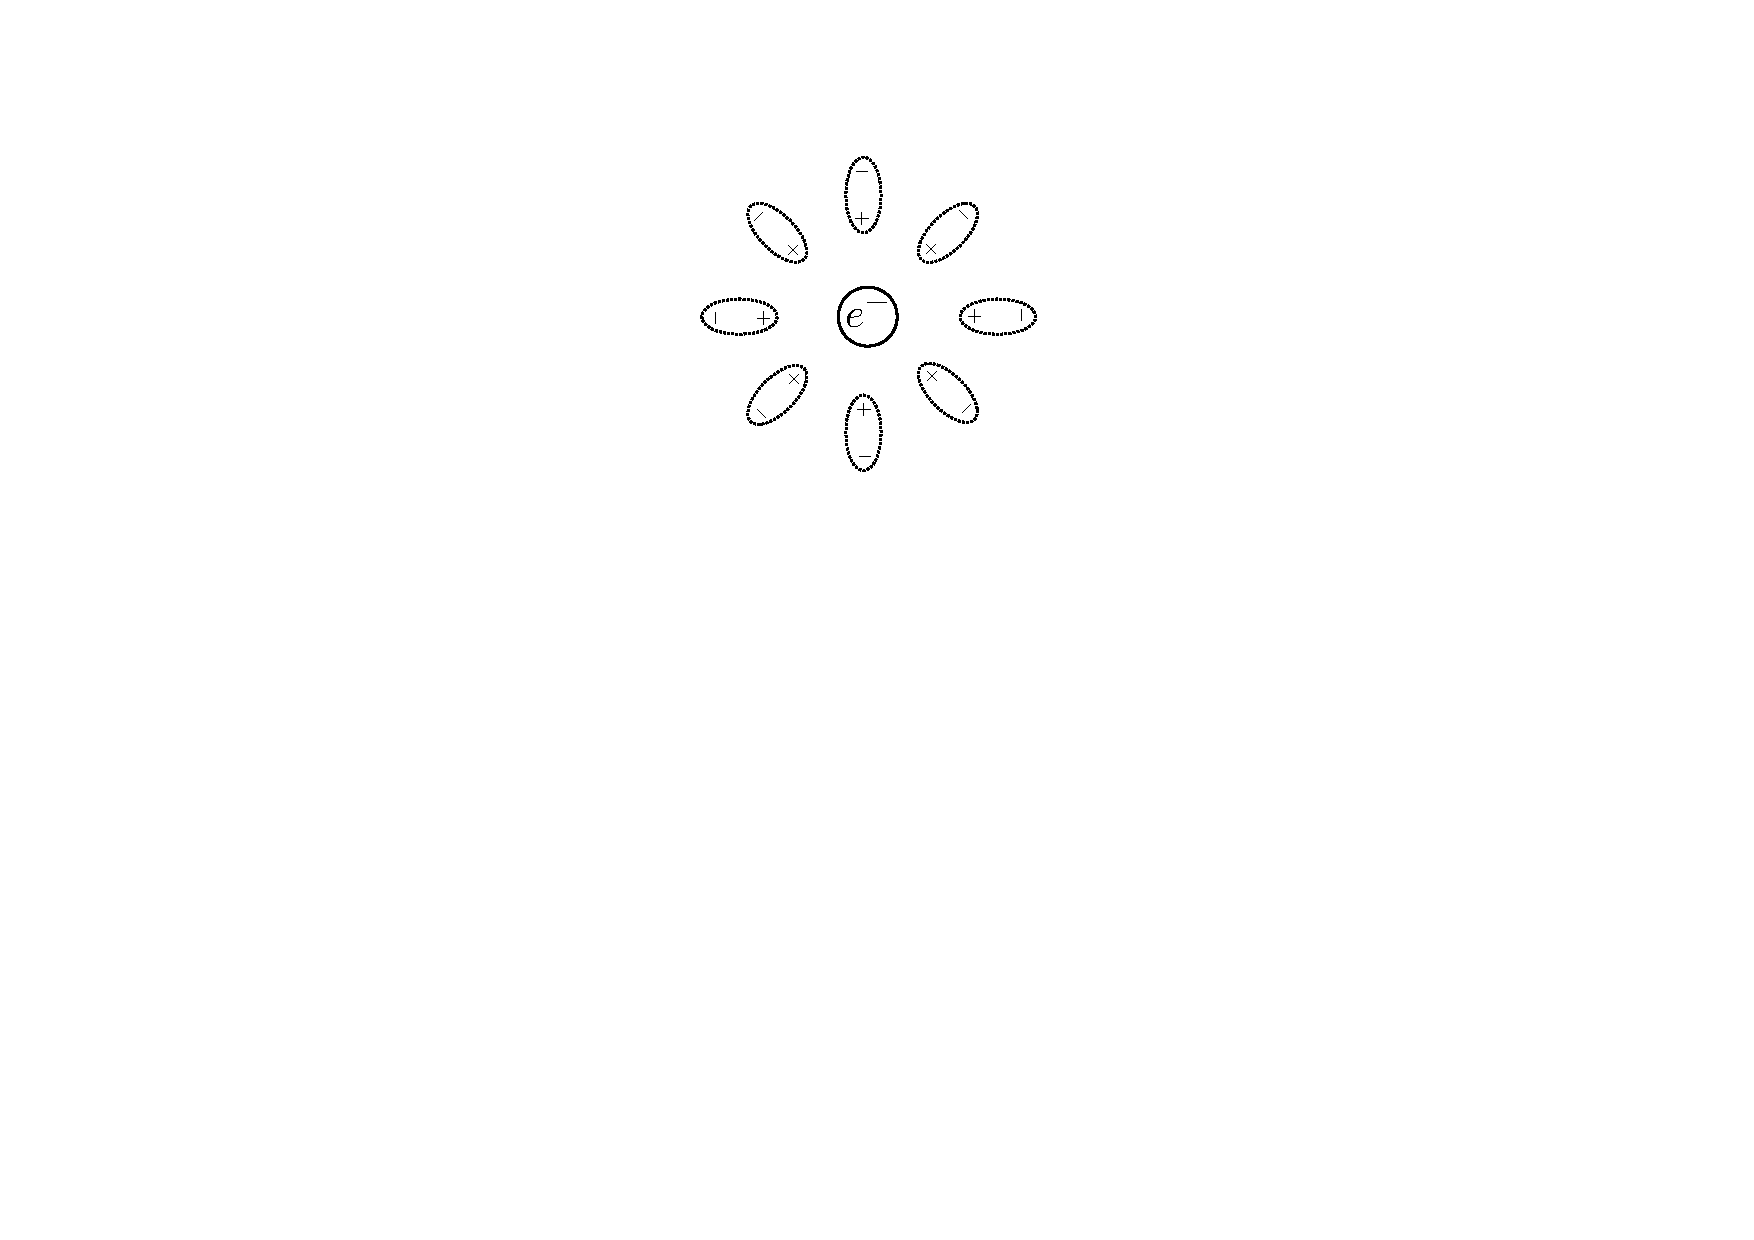
\includegraphics{QEDVacPol}
	\caption{QED vacuum polarisation}
	\label{fig:QEDVacPol}
\end{figure}
In contrast to QCD, calculating the beta function of QED shows that the coupling (the electric charge \(e\)) increases with the momentum scale, or equivalently decreases with distance. In the context of our discussion this can be understood by considering the vacuum as a dielectric medium, arising from virtual \(e^+e^-\) pairs as shown in Fig.~\ref{fig:QEDVacPol}. This polarisation cloud then screens the test charge such that the effective measured charge is less than the true value. As we penetrate deeper into the cloud, the test charge can be better resolved and we measure values ever closer to the true value. This is equivalent to probing at higher momentum transfers and thus represents the running coupling.\footnote{One somewhat interesting consequence of the naive perturbative calculation of the beta function in QED is the existence of the infamous Landau pole, or an infinite coupling, in the local limit \cite{Peskin:1995ev}. This signifies either a mathematical inconsistency in the theory if we assume that it should hold to arbitrary energy scales, or that this behaviour is somehow modified in the strong coupling regime.}

The considerations above originated in condensed matter physics where the background charge carriers are physical, mobile constituents of the material, for example as in plasmas, electrolytes, or electronic conductors. Thus one can make this more quantitative by characterising the medium by an electric permittivity \(\varepsilon\) and magnetic permeability \(\mu\), where
\begin{equation}
\varepsilon\mu=\frac{1}{c^2}=1,
\end{equation} 
and the speed of light \(c\) is in natural units. The permittivity and permeability describe the response of the medium to an applied external electric and magnetic field respectively, such as that imposed by the test charge in Fig.~\ref{fig:QEDVacPol}. A screening medium will diminish the electric field, or equivalently the effective charge, and has \(\varepsilon >1\). This corresponds to diamagnetism with \(\mu <1\). Conversely, a paramagnetic medium (\(\mu >1\)) will exhibit anti-screening of the electric field. When charges move in an external magnetic field, two competing effects take place to determine the regime in which the material will eventually settle \cite{Kharzeev:2002fm}:
\begin{itemize}
\item{Charges move in quantised orbits known as Landau levels. This creates a current which induces a magnetic field in the opposite direction to the external field, so this response is diamagnetic.}
\item{The spins of the charges align along the direction of the external magnetic field. This is a paramagnetic response.}
\end{itemize}
In QED the diamagnetic effect is dominant so the the vacuum polarisation screens the electric charge. It is important to note that we didn't need to consider the mediating gauge bosons of QED, photons, since they are chargeless.

A similar analysis can be performed in QCD to investigate colour screening. The arguments are identical but now one must consider colour charges instead of electric charges, and their corresponding chromo-electric and magnetic fields. One crucial difference arises, namely that the mediating gauge bosons now carry a colour charge. In particular, the virtual gluons act as permanent colour magnetic dipoles that align themselves with the external chromo-magnetic field, thus increasing its magnitude and producing \(\mu >1\). The anti-screening of the Yang-Mills vacuum can then be considered as paramagnetism. Furthermore, one can show that this effect is dominant over the screening due to virtual quark-antiquark pairs \cite{Nielsen:AF_spin}, and thus the full QCD vacuum is anti-screening.  
\subsection{Confinement}
\label{sec:confinement}
Perhaps the most fascinating, and notoriously impenetrable, aspect of QCD is \emph{confinement}. Formally, this is the statement that all observable states of finite energy are colour singlets -- colourless bound state hadrons. This manifests itself experimentally through the fact that asymptotically free (coloured) quarks and gluons have never been observed. It should be immediately emphasised that confinement is not simply the running coupling extrapolated into the low-energy hadronic regime. The so-called ``infrared slavery'' outlined in the previous section, where interactions grow increasingly strong, is alone not sufficient to explain and describe confinement \cite{Greensite:2003bk}. The phenomenon in much more intricate, and inherently non-perturbative. Indeed one of the well-known Millennium problems \cite{Clay_problem} is to rigorously prove confinement for (purely gluonic) Yang-Mills theory.

One of the most discussed and easily-visualised aspects of confinement is its manifestation in the quark-antiquark potential. In particular, in Euclidean field theory (see e.g. \cite{Rothe:1992nt}), the propagation of a quark-antiquark system in the infinite mass limit is described by an object \(W\brac{R,T}\) known as the Wilson loop with spatial extent \(R\) and temporal extent \(T\). At large times the expectation value of the Wilson loop asymptotes as
\begin{equation}
\label{eq:WilsonLoopExp}
\lim_{T\to\infty}\Braket{W\brac{R,T}}\sim\mathrm{exp}\brac{-V\brac{R}T}
\end{equation}
where \(V\brac{R}\) is the static potential acting between a heavy quark \(q\) and antiquark \(\bar{q}\). In the strong coupling regime one can demonstrate analytically that this potential grows linearly at large distances. This behaviour is also found for finite (anti-)quark mass using modern techniques with an improved definition of the static potential extracted from lattice calculations \cite{Burnier:2014ssa,Rothkopf:2011db,Bazavov:2011nk}. Why the linearly rising potential is confining can be understood qualitatively by considering so-called chromoelectric (colour) flux tubes shown in Fig.~\ref{fig:FluxTube}.
\begin{figure}[t]
	\centering
	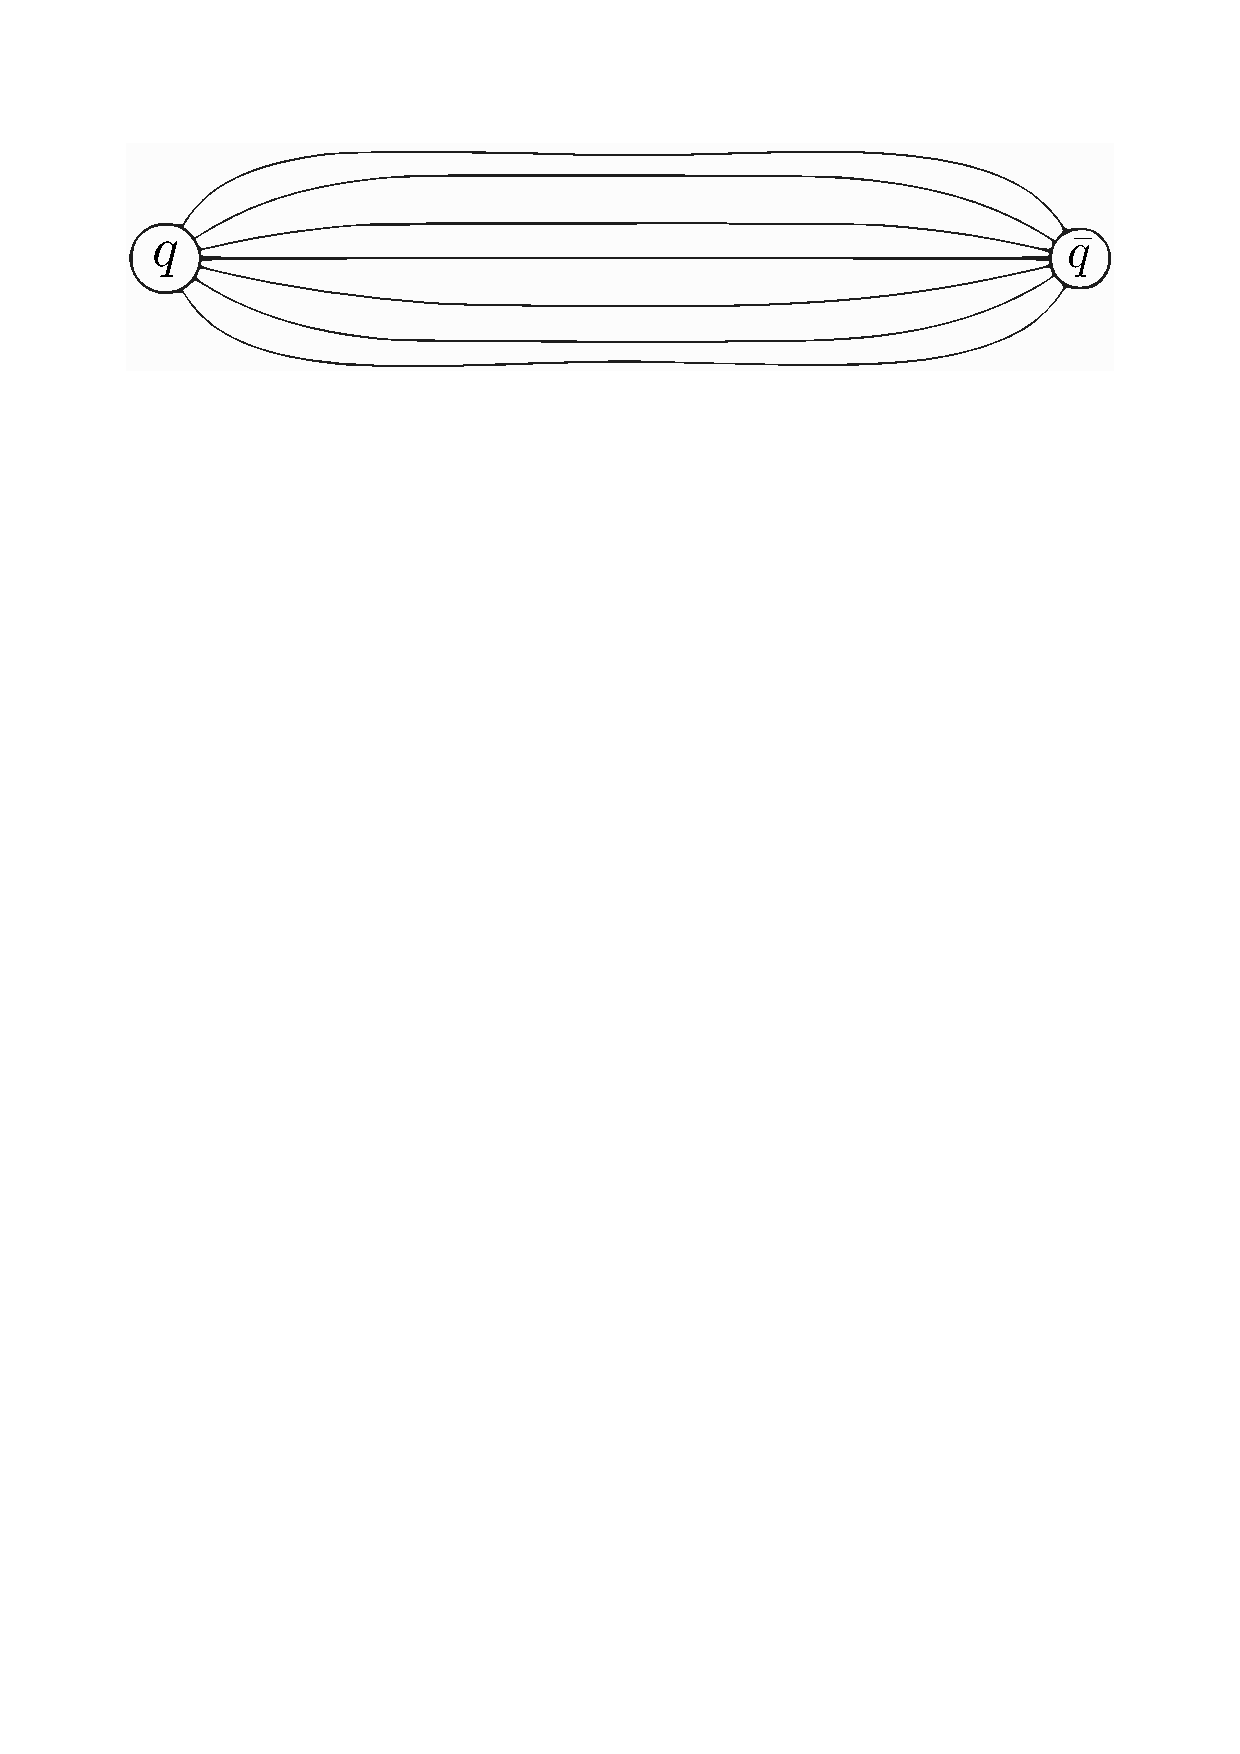
\includegraphics[width=\textwidth]{FluxTube}
	\caption{QCD Flux Tube}
	\label{fig:FluxTube}
\end{figure} 
In contrast to the more familiar dipole field lines of QED, the QCD field lines do not spread in space but instead remain concentrated within a narrow region due to the self interactions of the gluons. In this way the energy density within tube remains constant and so the total energy stored in the system increases linearly with the separation. If one imagines pulling the quark and antiquark apart, the interaction between them becomes stronger in a similar way to what happens with a spring. To increase the separation to infinity would require an infinite and thus unphysical amount of energy, so the linearly rising potential is considered confining. This explanation is intuitive but ultimately incomplete. The concept of a static potential is quantum mechanical and inherently non-relativistic. In reality, the potential is observed to flatten when it reaches a threshold value such that it becomes energetically favourable for the \(q\bar{q}\) bound state to dissolve into two heavy-light meson states. This phenomenon is known as \emph{string-breaking}, and will be discussed in more detail in Sec.~\ref{sec:quark_vac}.

A second, less rigorous way of interpreting confinement is through the language of vacuum polarisation developed in the previous section. There we concluded that the polarisation cloud of QCD takes an intrinsically small colour charge and acts in to increase its magnitude as we probe from further and further distances. However, the cloud itself is a soup of virtual particles and antiparticles all containing colour charge, so the energy of such a system seems to be increasing ad infinitum. The only way to resolve this divergence is to revisit the original assumption of an isolated colour source and conclude that this is unphysical. Since interpreting quarks and gluons as constituent parts of strongly-interacting bound states has been so successful in describing the hadron spectrum, one can think of colour-neutral objects as existing in such a way that the cloud of one source cancels the `anti-cloud' of another `anti-source' \cite{Wilczek_asymptoticfreedom}. Only these such objects can exist physically without requiring an infinite amount of energy, implying confinement.
\section{Thermodynamics of strongly interacting matter}
\label{sec:QCD_therm}
\onehalfspacing
Although we have not focused on the experimental verification of QCD, it should be emphasised that this theory has been extremely successful in describing a huge array of experimental results \cite{cahn_goldhaber_2009}. Most of these results come from particle accelerators and thus correspond to vacuum physics, however with growing confidence in QCD as the theory of strong interactions, more people became interested the \emph{in-medium} behaviour -- that is, at finite temperature and density. Today, the thermodynamics of QCD, or QCD under extreme conditions, is perhaps the most studied aspect of the theory. As well as posing many questions of purely academic interest, probing various regimes of in-medium QCD will also help elucidate the properties of some of the most exotic and yet physically-relevant phases of matter in the universe.
\subsection{Partition function}
\label{sec:QCD_therm_partfunc}
Formally, the equilibrium situation is described by a grand canonical partition function expressed via a Euclidean path integral \cite{kapusta_gale_2006}. Euclidean quantities are used ubiquitously in thermal field theory, as opposed to their Minkowskian counterparts of the zero-temperature vacuum case. The Euclidean Lagrangian \(\mathcal{L}^E_{QCD}\) can be found from the vacuum expression \eqref{eq:QCD_Lagr} by performing a Wick rotation \(\tau\to -it\) with \(\tau\in\mathbb{R}\), and replacing the Gamma matrices \(\gamma^\mu\) with the Euclidean versions \(\gamma^E_\mu\). The partition function is then given as \cite{Ding:2015ona}
\begin{equation}
\label{eq:tQCD_PartFunc}
Z\brac{T,V,\bm{\mu}}=\int\prod_{\mu}\mathcal{D}A_\mu\prod_{f=u,d,s...}\mathcal{D}\psi_f\mathcal{D}\bar{\psi}_f\;\mathrm{exp}\left[S_{E}\brac{T,V,\bm{\mu}}\right],
\end{equation}
with Euclidean action
\begin{equation}
\label{eq:tQCD_action}
S_E\brac{T,V,\bm{\mu}}=-\int_{0}^{\beta}\mathrm{d}x_{0}\int_{V}\mathrm{d}^3\mathbf{x}\;\mathcal{L}^E_{QCD}\brac{\bm{\mu}}.
\end{equation}
We have left the sum over spacetime and colour indices implicit, and introduced \(\beta=1/T\). As well as implicitly depending on the fundamental fields \(A,\psi,\bar{\psi}\) and quark masses \(\mathbf{m}=\brac{m_u,m_d,m_s,...}\), the action depends on a set of \(N_F\) chemical potentials \(\bm{\mu}=\brac{\mu_u,\mu_d,\mu_s,...}\) which we have made explicit. These couple to the conserved quark number currents via
\begin{equation}
\label{eq:tQCD_Lagr}
\mathcal{L}^E_{QCD}\brac{\bm{\mu}}=\mathcal{L}^E_{QCD}+\sum_{f=u,d,s...}\mu_f\bar{\psi}_f\gamma_0\psi_f.
\end{equation}
Just as in vacuum QFT, physical observables are obtained through
\begin{equation}
\label{eq:tQCD_obs}
\Braket{\mathcal{O}}=\frac{1}{Z\brac{T,V,\bm{\mu}}}\int\prod_{\mu}\mathcal{D}A_\mu\prod_{f=u,d,s...}\mathcal{D}\psi_f\mathcal{D}\bar{\psi}_f\;\mathcal{O}\;\mathrm{exp}\left[S_{E}\brac{T,V,\bm{\mu}}\right].
\end{equation}
Bulk thermodynamic quantities, such as pressure \(P\), energy density \(\epsilon\), and net quark number density \(n_f\), can then be calculated through standard relations:
\begin{align}
\label{eq:tQCD_P}\frac{P}{T^4}&=\frac{1}{VT^3}\;\mathrm{ln}Z\brac{T,V,\bm{\mu}},\\
\label{eq:tQCD_enden}\frac{\epsilon}{T^4}&=-\frac{1}{VT^3}\frac{\partial\;\mathrm{ln}Z\brac{T,V,\bm{\mu}}}{\partial\beta}\bigg\rvert_{\bm{\mu},T\;\;\mathrm{fixed}},\\
\label{eq:tQCD_qn}\frac{n_f}{T^3}&=\frac{1}{VT^3}\frac{\partial\;\mathrm{ln}Z\brac{T,V,\bm{\mu}}}{\partial\hat{\mu}_f},
\end{align}
where \(\hat{\mu}_f=\mu_f/T\) is the chemical potential in units of temperature. 

The chemical potential will play a crucial role in the remainder of this thesis. In particular, the baryon chemical potential is defined \(\mu_B=\sum_f \mu_f\) which in general will depend on the number of active flavours being probed at the relevant energy scale. There is no process in QCD that can change the number of baryons \(N_B\) minus the number of anti-baryons \(\bar{N}_B\); the quantum number \(B=N_B-\bar{N}_B\) called baryon number is conserved. Since an (anti-)baryon is made of three (anti-)quarks, quarks and anti-quarks have \(B=\pm\frac{1}{3}\) respectively. Analysing the system in the grand canonical ensemble \(\Omega\brac{T,V,\mu_B}=E-TS-\mu_BB\), where \(E\) is the total energy and \(S\) the entropy, allows the baryon number to vary. Thermodynamic equilibrium is achieved when \(\Omega\) is minimised, in which case we can associate \(\mu_B\) as the increase in energy whenever \(B\) increases by one. In the grand canonical ensemble \(\mu_B\) can be thought of as a control parameter such that the baryon density \(n_B=B/V\) is a derived quantity that depends on the details of the equation of state, \(n_B=n_B\brac{T,\mu_B}\) \cite{2001ConPh..42..209H}. 
\subsection{Phase diagram}
\label{sec:QCD_phase}
\begin{figure}[t]
	\centering
	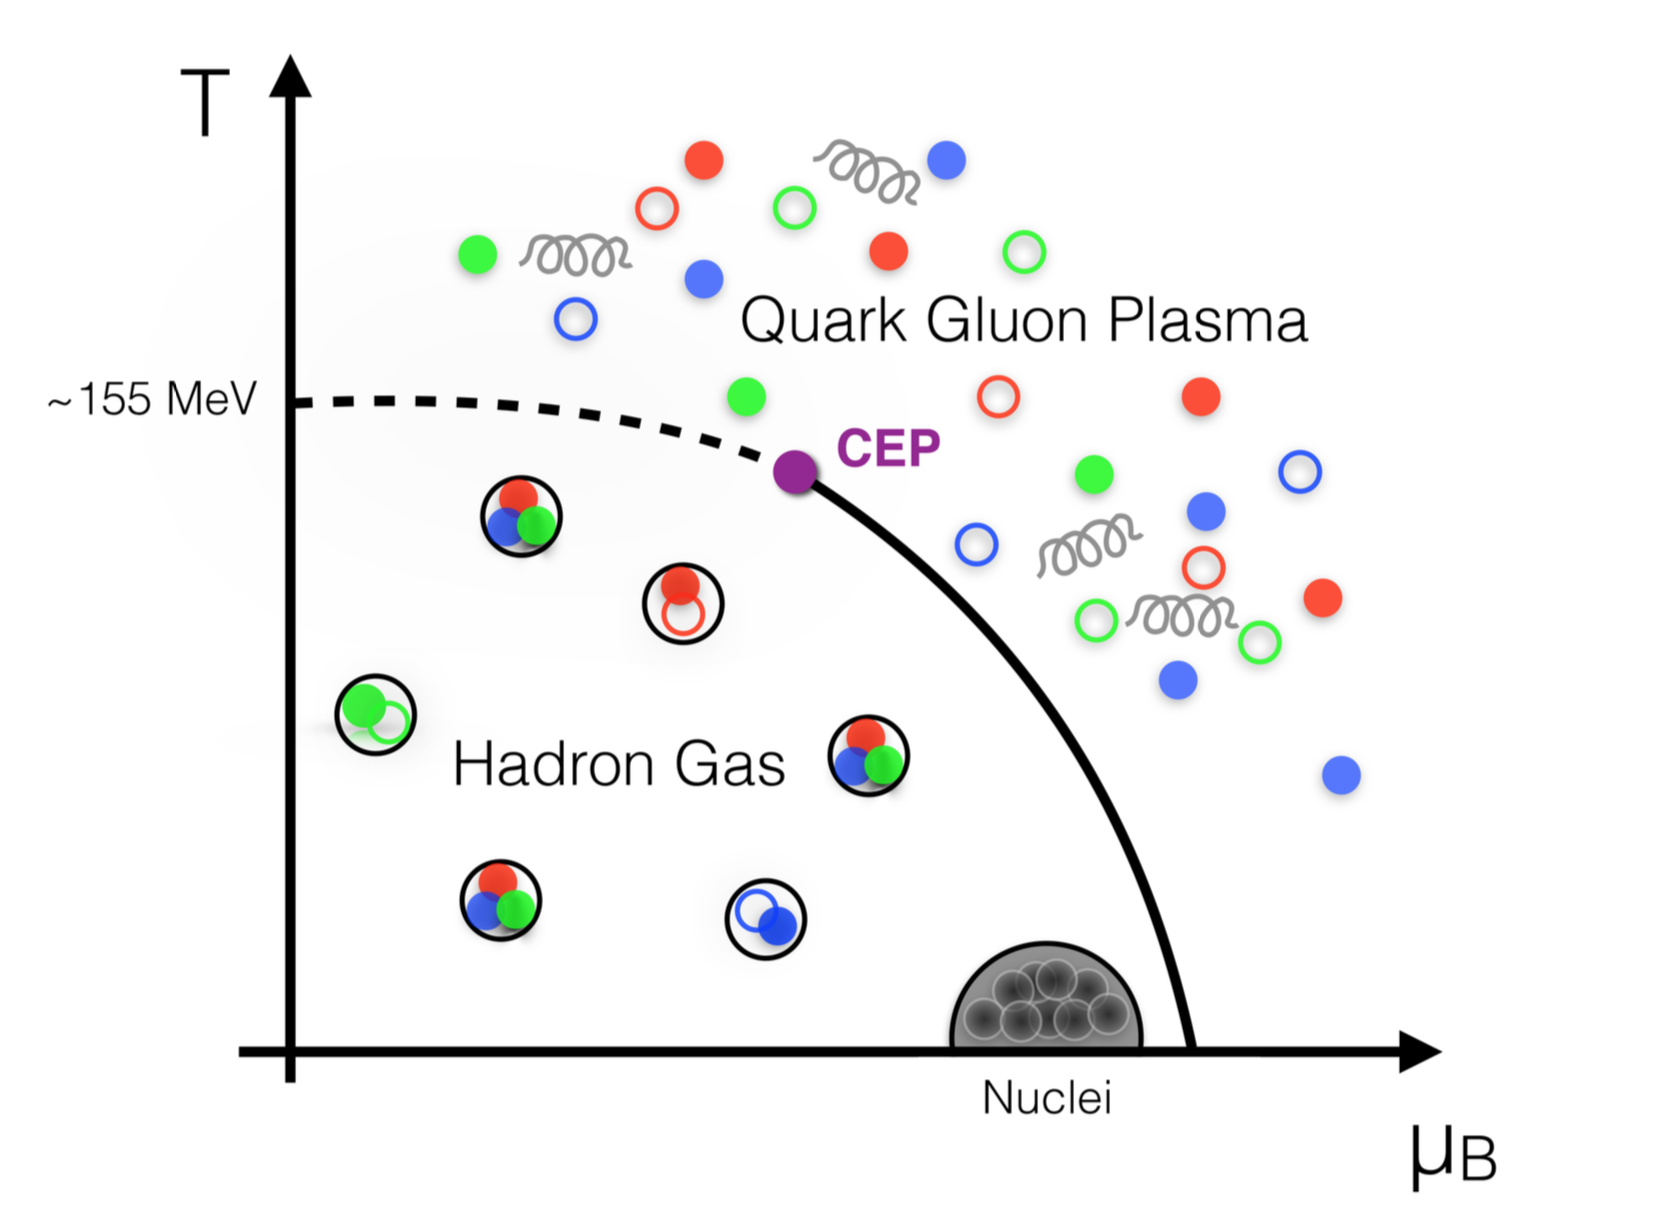
\includegraphics[width=\textwidth]{QCDphase}
	\caption{A qualitative QCD phase diagram.}\label{fig:QCDphasediag}
\end{figure}
We now provide a short overview of the currently understood phase diagram of strongly interacting matter, shown in Fig.~\ref{fig:QCDphasediag}. For clarity, the most prominent features will be given in a listed format. The reader can consult \cite{Rischke:2003mt} and references therein for a more detailed account.
\\
\\
\textbf{Liquid-Gas transition.} We begin exploring the phase diagram at strictly vanishing temperature. Increasing the chemical potential (quark density) corresponds to injecting pions (\(q\bar{q}\) bound states of up and down flavours) into the system. This situation will persist until \(\mu_B\) reaches the value of the nucleon (proton or neutron) rest mass minus the binding energy per nucleon in nuclear matter. At this point, \(\mu_{B,0}\simeq 922\mathrm{MeV}\), it becomes energetically favourable to populate the ground state with a bound nucleon fluid. The baryon density then jumps form zero to \(n_{B,0}\simeq 0.17\mathrm{fm^{-3}}\), indicating a first order phase transition. From continuity arguments this behaviour is expected to remain at small finite temperatures, and a coexistence line emerges from \(\mu_{B,0}\) ending in a critical point at temperatures of around \(10\mathrm{MeV}\) \cite{Rischke:2003mt}. This is analogous to the liquid-gas transition of water, with pions playing the role of gaseous `molecules' and nucleons corresponding to liquid `droplets'. As such, it is known as the nuclear liquid-gas transition.\\
\textbf{Quark matter \& colour superconductivity.} Remaining on the \(T=0\) axis, we now ask what happens if we increase the chemical potential further. Naively, we would expect that the degrees of freedom would transition from baryons to quarks at densities where the volume per baryon equals the baryon volume. Different estimates place this at around \(\mu_{sc}\simeq 1100-1500\mathrm{MeV}\) \cite{2001ConPh..42..209H}. In order to reach these densities a huge external pressure is required; the most likely physical source are the gravitational forces present in compact astrophysical objects such as neutron stares. Furthermore, it is expecting that quark matter becomes a colour superconductor in this regime due to the condensation of quark Cooper pairs living near the Fermi surface \cite{Alford:2001dt}, however this is very much still an active area of research. \\
\textbf{Deconfinement Transition.} Based on the discussion of asymptotic freedom in Sec.~\ref{sec:QCD_run_free}, one would expect that by inserting more energy into the system by increasing the temperature, the (anti-)quarks would become more weakly bound and at high enough temperatures the relevant degrees of freedom would transform from hadrons to deconfined (anti-)quarks and gluons. Exactly this line of thought led Cabbibo and Parisi \cite{Cabibbo:1975ig} to interpret Hagedorn's limiting temperature of hadronic matter \cite{Hagedorn:1965st} as signalling a transition to a new state of matter, later coined the quark gluon plasma by Shuryak \cite{Shuryak:1978ij}. Modern research aims to discern the properties of this transition -- at which temperatures and densities does it occur and whether a smooth crossover exists or a phase transition exhibiting critical behaviour -- and to understand the emergent phenomena exhibited by the QGP. These are deep questions that probe the underlying symmetries of QCD, for example the spontaneous breaking of chiral symmetry \cite{Martinez:2013xka}, and will be addressed further in the following sections.
\subsection{Quark Gluon Plasma}
\label{sec:QGP}
The quark gluon plasma, as a deconfined `hot soup' of quarks and gluons, is an inherently non-perturbative phenomenon. As such, it is somewhat less amenable to the usual perturbative expansions that are very successful in describing vacuum physics. However, various theoretical approaches do exist that continue to provide valid insights. The most important in the scope of this thesis will be that of \emph{weak-coupling}. Qualitatively speaking, the argument is straightforward: asymptotic freedom would suggest that the high temperature regime is weakly interacting. Indeed, if we momentarily assume a non-interacting gas of massless particles, the Stefan-Boltzmann law allows one to calculate the pressure and energy density:
\begin{equation}
\label{eq:SBres}
\epsilon=g\frac{\pi^2}{30}T^4\begin{cases}
    1 & \text{bosons}\\
    7/8 & \text{fermions}
  \end{cases},\quad P=\epsilon/3,
\end{equation}
where \(g\) is the number of degrees of freedom. For the case of (assumed massless) quarks and gluons, we have \(g_q=12N_F\) (2 spin states, 3 colour states, 2 particle/anti-particle states) and \(g_g=16\) (2 helicity states and 8 colour states). Assuming \(N_F=3=u,d,s\) this gives
\begin{equation}
\label{eq:SB_pres}
\epsilon_{SB}=\frac{95}{2}\frac{\pi^2}{30}T^4.
\end{equation}
This result is displayed in Fig.~\ref{fig:lattice_en_den}, which also shows the lattice results to be discussed in Sec.~\ref{sec:latticeQCD}. Although overestimating the calculated value by around 20\%, it indicates that even considering the QGP a classical non-interacting gas of massless particles, known as the ideal QGP, is a reasonable starting point for the determination of some quantities. It can also be noted here that the jump in energy density in Fig.~\ref{fig:lattice_en_den}, reminiscent of a CLASSICAL PHASE TRANSITION, can be attributed to a quantitative change in the number of degrees of freedom from a pion gas to a deconfined medium.\footnote{Indeed one can make an estimate of the transition temperature using such considerations and a crude bag-model for hadrons, the result of which turns out to be surprisingly accurate \cite{2001ConPh..42..209H}.} Switching on interactions appears to only slightly modify this simple behaviour, however the calculation of QGP thermodynamic quantities using weak-coupling techniques was for a long time plagued by many difficulties. A strict expansion in powers of the coupling constant converges poorly, with alternating contributions oscillating wildly \cite{Blaizot:2003tw}. In general, a small coupling does not permit a perturbative expansion at finite temperature \cite{Arnold:2007pg}, due to the existence of thermal fluctuations. In quantities such as the plasma free energy, or as will be seen in Sec.~\ref{sec:med_pot} the screening length, the coefficients of a weak coupling expansion become truly non-perturbative beyond a calculable order. Whether the weak coupling approach is accurate is thus decided by which momentum scale (controlling the magnitude of thermal fluctuations) is dominant for the quantity under consideration \cite{Blaizot:2003tw}. Indeed there is active research in investigating a strongly-coupled QGP \cite{Gyulassy:2004zy}, with modern developments making use of the AdS/CFT correspondence which can be used to map strongly-coupled quantum field theories to a weakly-coupled theory of quantum gravity formulated in terms of string theory \cite{CasalderreySolana:2011us}.
\subsection{Lattice QCD}
\label{sec:latticeQCD}
The Euclidean formulation of finite temperature field theory lends itself naturally to lattice QCD, which remains the only first-principles tool for studying the inherently non-perturbative nature of the theory under extreme conditions. First suggested by Kenneth Wilson in 1974 \cite{Wilson:1974sk}, lattice gauge theory provides a regularisation scheme for QCD by introducing a finite real-space lattice spacing, and thus an ultraviolet momentum cut-off. In doing so, spacetime is discretised and the path integral becomes a finite, high-dimensional integral over appropriately defined fermion and gauge fields (see e.g. \cite{Rothe:1992nt}). The intricate process of taking the continuum limit and achieving physical results is performed by sending the lattice spacing to zero and ensuring no lattice artefacts (such as cut-off dependencies) remain in the relevant observables. With ever more efficient algorithms running on ever more powerful supercomputers, lattice calculations have recently been able to give quantitative predictions. For massless quarks and vanishing chemical potentials, these calculations have demonstrated the existence of a first order transition at a critical temperature of around \(173\) MeV \cite{Martinez:2013xka}. This can be seen in the behaviour of the energy density in Fig.~\ref{fig:lattice_en_den}. At physical quark masses, the critical behaviour fades away and is replaced by a crossover transition. The crossover temperature is somewhat more difficult to define, and different methods have determined a value in the region of \(150-200\) MeV. 
\begin{figure}[t]
	\centering
	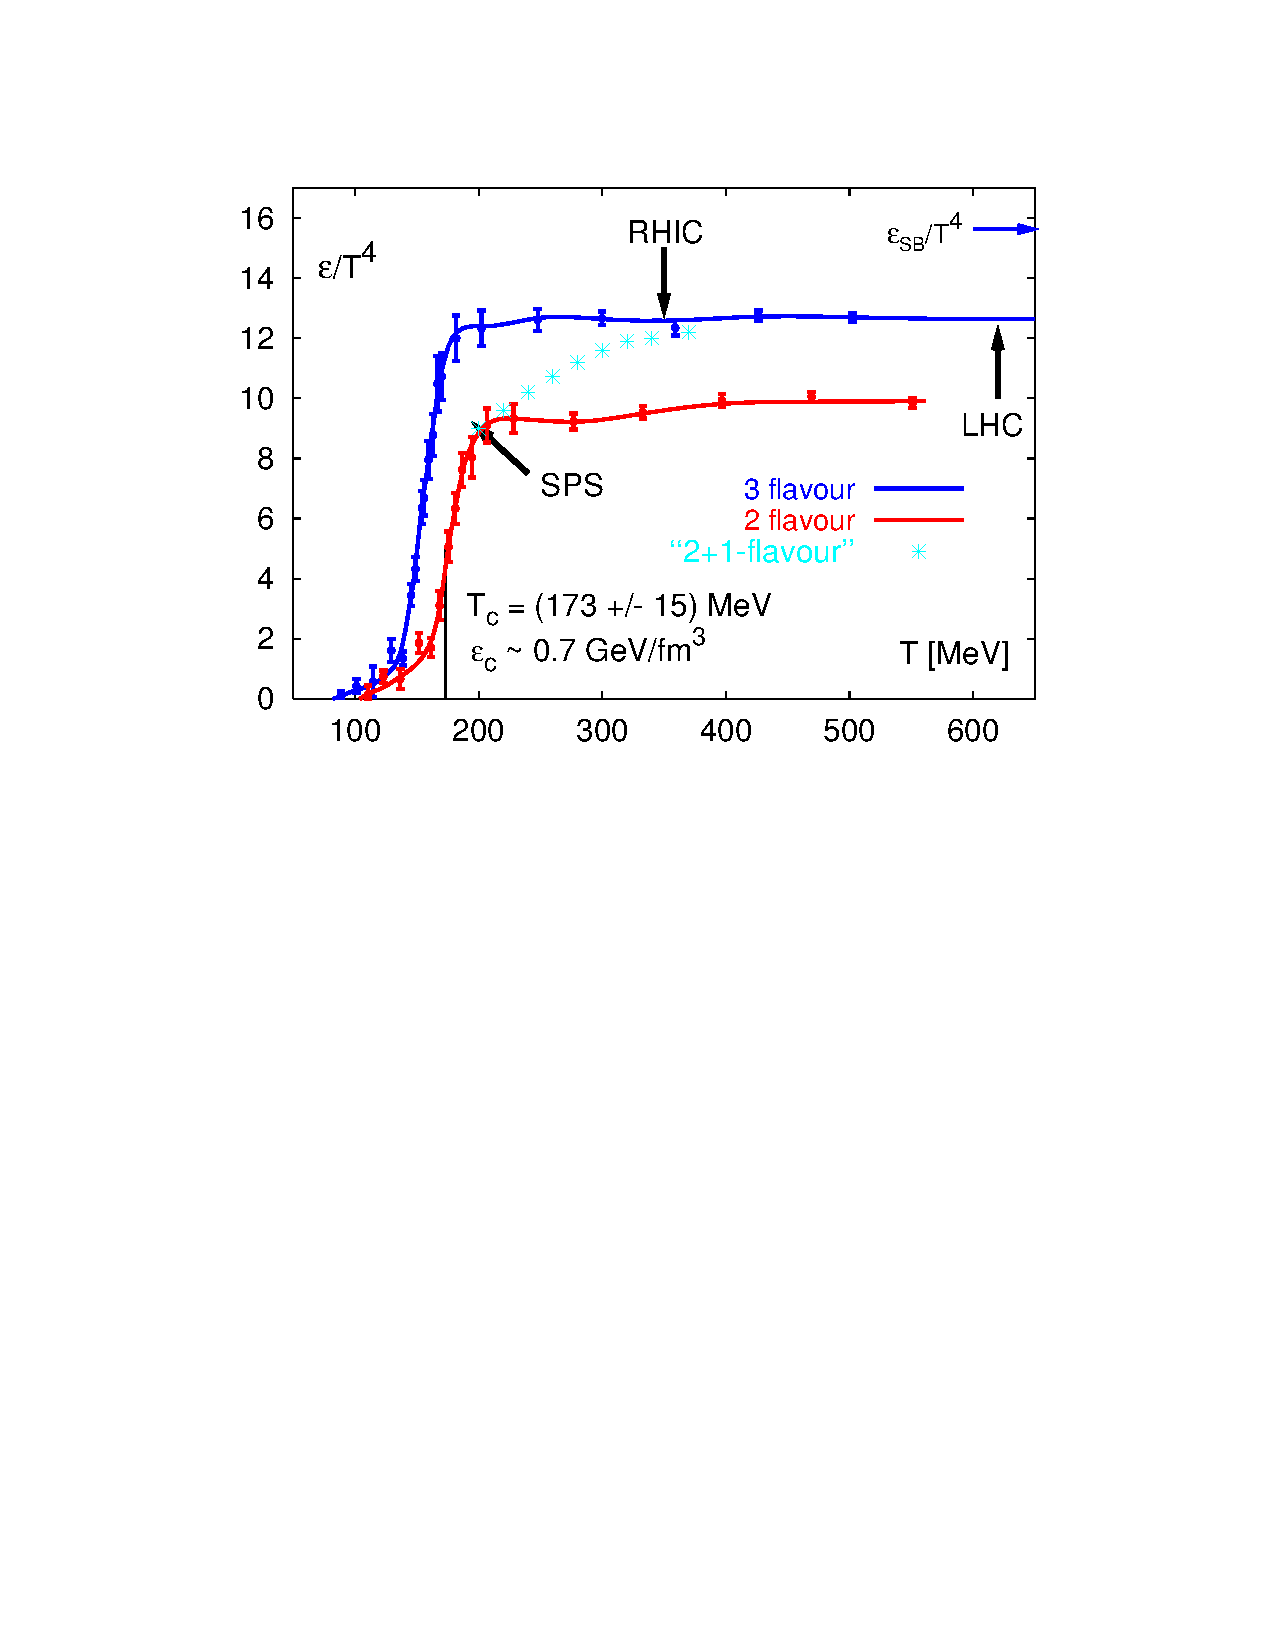
\includegraphics[width=\textwidth]{QCD_lat_enden}
	\caption{The temperature dependence of the energy density \eqref{eq:tQCD_enden} from lattice QCD at vanishing baryon chemical potentual \cite{Martinez:2013xka}. Calculations are performed for two massless quarks, three massless quarks, and two massless quarks plus one (\(s\)) of physical mass (2+1).}\label{fig:lattice_en_den}
\end{figure}

Throughout the rest of this thesis we take the crossover temperature as that determined from chiral order parameter calculations, \(T_C\simeq155\) MeV.
\section{Quarkonium in vacuum}
\label{sec:quark_vac}
\onehalfspacing
\section{Heavy Ion collisions}
\label{sec:quark_HIC}
\onehalfspacing
\chapter{The in-medium potential}
\label{sec:med_pot}
\onehalfspacing
\chapter{Quarkonium Phenomenology}
\label{sec:quark_pheno}
\onehalfspacing
\chapter{Conclusion}
\label{sec:conc}
\onehalfspacing

%\begin{appendices}
%\chapter{Thermal field theory}
%\chapter{Debye mass derivation}
%\chapter{Schwinger-Keldysh formalism}
%\end{appendices}

\bibliography{references}

\chapter*{Acknowledgements}


\cleardoublepage
\setlength{\parindent}{0em}

Erkl\"{a}rung:\par
\vspace{3\baselineskip}
Ich versichere, dass ich diese Arbeit selbstst\"{a}ndig verfasst habe und keine
anderen als die angegebenen Quellen und Hilfsmittel benutzt habe.\par
\vspace{5\baselineskip}
Heidelberg, den (Datum)\hspace{3cm}\dotfill


\end{document}
